\section{Audio Processing Unit (APU)}

{\it Note: this section is even less complete than the others}

The APU is a lightweight processing core, designed to synthesise polyphonic audio, stream PCM or ADPCM audio from the system, or a mixture of the two, whilst blending/panning the audio channels. It runs in hard real time: each audio sample is calculated in one sample period, so no data buffering is required between APU and DACs. The design goals are:

\begin{enumerate}
	\item Low resource utilisation ($~100$ LUTs for the processing core)
	\item Output 48 kSa/s 8-bit stereo audio with a 12 MHz clock
	\item Provide similar interface to an 8-bit era games console with default APU code, so no programming required
	\item Streaming PCM audio from the system should be trivial (ring buffer + IRQ)
	\item Be fun to program: very focused on a single task, so quirky but easy to learn
\end{enumerate}

\subsection*{Architectural Overview}

\subsubsection*{Memory Architecture}

The APU is designed around a pair of iCE40 block RAMs: each is 16 bits wide by 256 entries deep, and has an independent read port and write port. The architecture and microarchitecture are designed around these parameters, for efficient use of the memory, and in particular for high utilisation of the memory ports. Figure \ref{diagram:apu_mem_arch} shows this in overview.

\begin{figure}[H]
\centering
\caption{Audio processing unit memory architecture}
\label{diagram:ppu_arch}
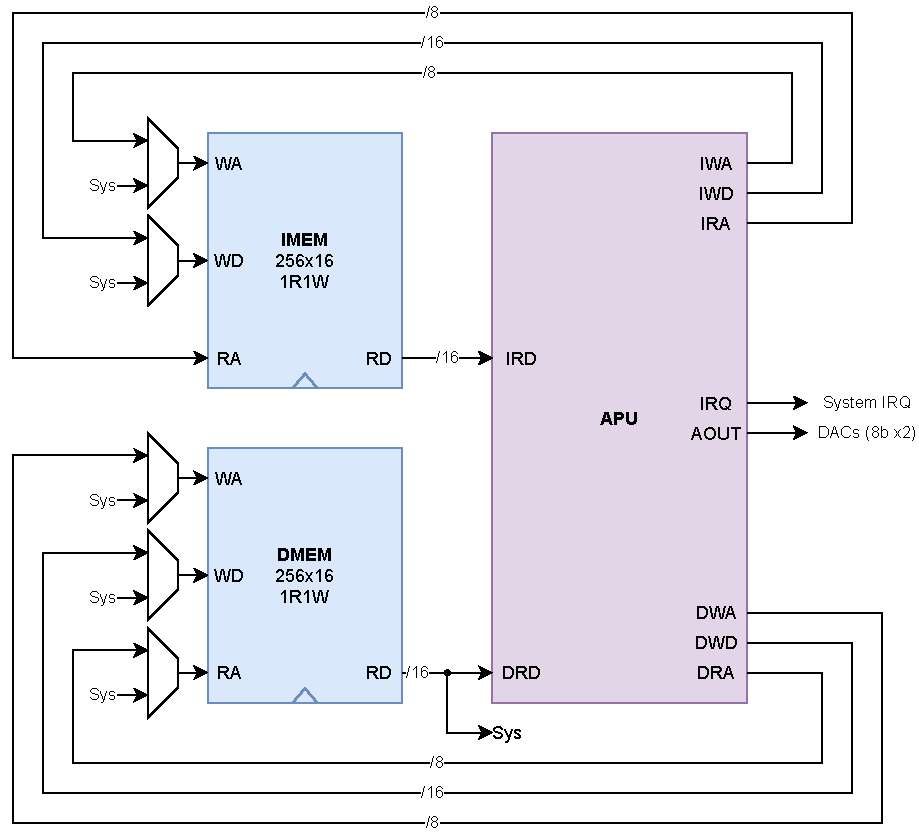
\includegraphics[width=0.6\textwidth]{diagrams/apu_mem_arch.pdf}
\end{figure}


\begin{itemize}
	\item IMEM:
	\begin{itemize}
		\item Contains the APU program instructions. Each instruction is 16 bits in size.
		\item Upper 8 slots contain a copy of the APU's general purpose registers
		\item The system has write-only access when the APU is halted, and no access when the APU is running
	\end{itemize}
	\item DMEM:
	\begin{itemize}
		\item Contains sample ring buffers used for wave tables or for buffering PCM data from the system
		\item Contains program temporary variables that don't fit into registers or need to be indexed
		\item Upper 8 slots contain a copy of the APU's general purpose registers
		\item The system has read-write access at all times, at a lower priority than the APU (system access stalls when the APU is accessing DMEM)
	\end{itemize}
\end{itemize}

8 general-purpose registers are available to APU programs. The register contents are mirrored across IMEM and DMEM, so that two independent register reads can take place simultaneously. Register writeback of one instruction is overlapped with instruction fetch of the next instruction. A typical register-to-register instruction (e.g. an add) executes in two cycles, performs 3 memory reads and 2 memory writes.

\subsubsection*{Arithmetic}

There are two data types used by APU instructions:

\begin{itemize}
	\item 16-bit integers
	\item Packed pairs of 8-bit integers (SIMD)
\end{itemize}

The former is useful for control variables and for phase accumulation of digital oscillators. The latter is used for SIMD processing of stereo sampling pairs. All 8-bit arithmetic is signed-saturating. 16-bit arithmetic can generally be either signed-saturating or normal modular arithmetic.

\subsubsection*{Input/Output}

The APU performs all calculations necessary to produce a 2$\times$8-bit stereo sample pair, then outputs this to the external DACs (probably some kind of sigma delta thing) with an {\tt out} instruction. The APU then stalls until the end of the audio sample period, whereupon it begins calculating the next samples.

For PCM sample streaming, the APU accesses ring buffers in DMEM, in the same way that it access DMEM wavetables for local synthesis. The system tops up the ring buffers by writing to DMEM, triggered by APU interrupts.

The {\tt irq} instruction can generate a system interrupt, which is mainly useful for half-empty or quarter-empty interrupts for PCM ring buffers.

\subsection{Instruction Set}

The two main instruction formats are:

{\bf R format}

\begin{bytefield}[endianness=big]{16}
\bitheader{0,4,5,7,8,10,11,15} \\
\bitbox{5}{{\tt opcode}} \bitbox{3}{{\tt rd}} \bitbox{3}{{\tt rs}} \bitbox{5}{\reservedfield}
\end{bytefield}

{\bf I format}

\begin{bytefield}[endianness=big]{16}
\bitheader{0,7,8,10,11,15} \\
\bitbox{5}{{\tt opcode}} \bitbox{3}{{\tt rd}} \bitbox{8}{{\tt imm}}
\end{bytefield}

\subsection*{Example Programs}

\subsubsection*{Wave channel}

\begin{lstlisting}
.imem                     ; List instruction memory contents
	ld r1, [#freq]        ; Initialise frequency from data memory
	li r0, #0             ; Initialise phase to 0
loop:
	addm16 r0, r1         ; Modular 16-bit addition to advance phase
	ldw r2, [r0, #sine]   ; Look up 2x8-bit samples in sine wave table
	out r2                ; Output samples to DAC, stall until next sample
	b loop                ; Repeat forever

.dmem                     ; List data memory contents
sine:
	...
freq:
	.hword 0x1234
\end{lstlisting}

\subsubsection{Wave channel, controllable frequency}

\begin{lstlisting}
.imem
loop:
	ld r1, [#freq]        ; Fetch frequency stored in memory
	ll r0, [#phase]       ; Fetch phase stored in memory, and set exclusive flag
	addm16 r0, r1         ; Increment phase by frequency
	sc r0, [#phase]       ; Store phase back into memory if still exclusive
	ldw r0, [r0, #sine]   ; Load wave sample from sine table
	out r0                ; Output 2x8-bit samples from r0
	b loop                ; Always jump to loop

.dmem
sine:
	...
freq:
	.hword 0x1234
phase:
	.hword 0
\end{lstlisting} 

\subsubsection{Wave channel, controllable volume with decay}

\begin{lstlisting}
.imem
loop:
	ld r1, [#freq]       ; Atomic update phase based on frequency
	ll r0, [#phase]
	addm16 r0, r1
	sc r0, [#phase]
	ld r2, [#decay]      ; Atomic update volume based on linear decay
	ll r1, [#volume]
	sub16 r1, r2
	sc r1, [#volume]
	ldw r0, [r0, #sine]  ; Look up wave table based on phase
	movhl r1, r1         ; Duplicate upper byte of volume
	mul48 r0, r1         ; Multiply each sample by 4 volume MSBs
	out
	b loop

.dmem
sine:
	...
freq:
	.hword 0x1234
phase:
	.hword 0
decay:
	.hword 0xabcd
volume:
	.hword 0
\end{lstlisting}

\subsubsection{Multiple wave channels}

